%%%%%%%%%%%%%%%%%%%%%%%%%%%%%%%%%%%%%%%%%%%%%%%%%%%%%%%%%%%%%%%%%%%%%%%%%%%%%
%
%  System        : 
%  Module        : 
%  Object Name   : $RCSfile$
%  Revision      : $Revision$
%  Date          : $Date$
%  Author        : $Author$
%  Created By    : Robert Heller
%  Created       : Sat Apr 15 10:30:00 2023
%  Last Modified : <230415.1030>
%
%  Description 
%
%  Notes
%
%  History
% 
%%%%%%%%%%%%%%%%%%%%%%%%%%%%%%%%%%%%%%%%%%%%%%%%%%%%%%%%%%%%%%%%%%%%%%%%%%%%%
%
%    Copyright (C) 2023  Robert Heller D/B/A Deepwoods Software
%			51 Locke Hill Road
%			Wendell, MA 01379-9728
%
%    This program is free software; you can redistribute it and/or modify
%    it under the terms of the GNU General Public License as published by
%    the Free Software Foundation; either version 2 of the License, or
%    (at your option) any later version.
%
%    This program is distributed in the hope that it will be useful,
%    but WITHOUT ANY WARRANTY; without even the implied warranty of
%    MERCHANTABILITY or FITNESS FOR A PARTICULAR PURPOSE.  See the
%    GNU General Public License for more details.
%
%    You should have received a copy of the GNU General Public License
%    along with this program; if not, write to the Free Software
%    Foundation, Inc., 675 Mass Ave, Cambridge, MA 02139, USA.
%
% 
%
%%%%%%%%%%%%%%%%%%%%%%%%%%%%%%%%%%%%%%%%%%%%%%%%%%%%%%%%%%%%%%%%%%%%%%%%%%%%%

\section{Assembly}
\begin{figure}[hbpt]\begin{centering}%
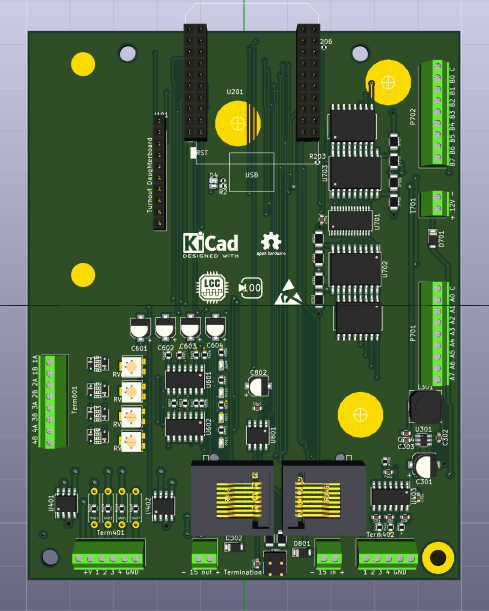
\includegraphics[width=4in]{ESP32-T7S3-MultiFunctionUniversalTurnout.png}
\caption{3D image of the ESP32 T7S3 MultiFunctionUniversalTurnout board}
\end{centering}\end{figure}
\begin{figure}[hbpt]\begin{centering}%
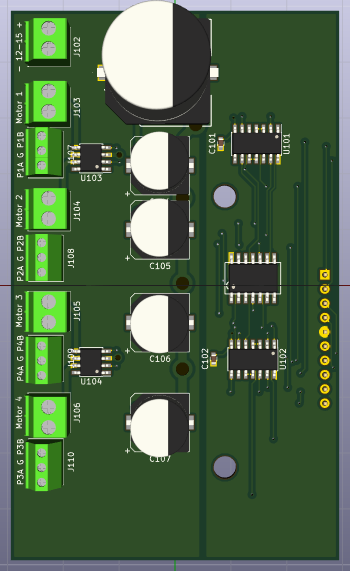
\includegraphics[height=3in]{SC-DaughterBoard.png}
\caption{3D image of the Single Coil Turnout driver daughter board}
\end{centering}\end{figure}
\begin{figure}[hbpt]\begin{centering}%
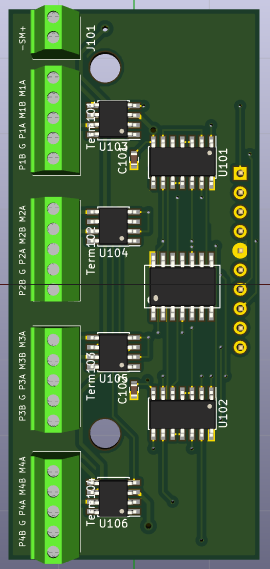
\includegraphics[height=3in]{SM-DaughterBoard.png}
\caption{3D image of the Stall Motor driver daughter board}
\end{centering}\end{figure}
\begin{figure}[hbpt]\begin{centering}%
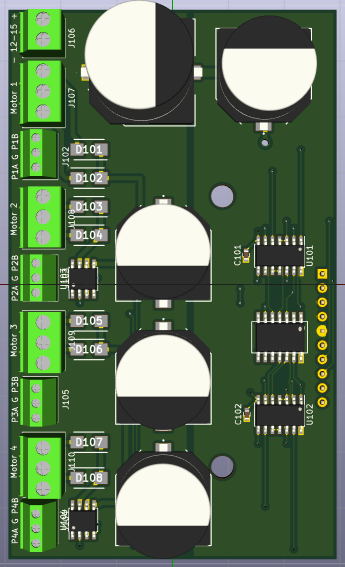
\includegraphics[height=3in]{TC-DaughterBoard.png}
\caption{3D image of the Twin Coil driver daughter board}
\end{centering}\end{figure}
\begin{figure}[hbpt]\begin{centering}%
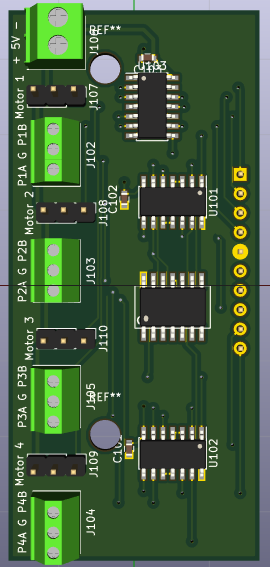
\includegraphics[height=3in]{TS-DaughterBoard.png}
\caption{3D image of the Servo driver daughter board}
\end{centering}\end{figure}
\clearpage

The boards have all of the SMD parts factory installed. Only the through-hole
parts are not soldered to the board. These are the RJ45 Jacks, the Termination
Jumper, the turnout daughter board header, the min32 headers, the daughter
board support standoffs, and the terminal blocks. The daughter boards also
have all of their SMD parts factory installed, and just needs their terminal
blocks and board inter-connect pin array headers installed. These are all easy
to solder parts. Make sure the headers and terminal blocks are fully seated
and square to the boards. A simple trick is to solder one pin and then while
pressing the part to the board, reheat that one pin's solder pad and snapping
the part to the board and holding it tight and square to the board as the
solder cools. Important: make sure the wire entry holes in the terminal blocks
are facing the edge of the board! The RJ45 Jacks cannot be installed wrong
(they have orientation pins). Start with the shortest parts and work up to the
tallest. Note: the pin array on the daughter board goes on the bottom of the
board and is soldered on the top side.

%% Need photo of a daughter board's pin array.

\begin{figure}[hbpt]\begin{centering}%
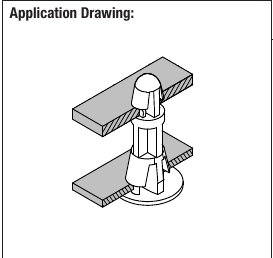
\includegraphics{NylonStandoffInstall.png}
\caption{Nylon Standoff Installation}
\end{centering}\end{figure}

The daughter boards are supported with a pair of nylon standoffs.  These are 
pushed through from the bottom of the main board.

You also need to solder the 2x10 pin headers to the bottom of the T7S3 board.

%% Add photo

Once all of the soldering is done, the T7S3 can be installed on the main board.
The WiFi antenna extends beyond the top of the board, with the T7S3's USB 
connector facing into the center of the board.  The daughter board's pin array 
goes in the socket header on the main board and there are two holes in the 
daughter board that engage the nylon standoffs.

%% Need a photo of a daughter board being installed on the main board 
%% and probably one of the T7S3 installed on the main board.

\clearpage
